

\chapter{Collatz SRS Analysis} \label{sec:hardnessrewriterules}
\hl{Now that we have explained Heule's and Aaronson's attempts to solve the Collatz Conjecture, we focus on analyzing the Collatz SRS further. We do so by simulating the Collatz SRS and various modifications of it in order to analyze the number of steps these SRSes take.} First, we discuss a program we created that replays the Collatz SRS for any input number, which is used throughout this chapter. We then attempt to establish a reasonable bound for number of rewrite steps by comparing classical hardness records from Chapter~\ref{sec:subhrdnspred}. We use this bound to compute reasonable hardness measures for modifications of the Collatz SRS that align with unproven Base 8 Collatz Variants. Finally, we explore a modification to Aaronson's rewrite system which reduces rewrite steps.
\section{Simulating the Collatz SRS} \label{subsec:rewritecomp}
We wrote a program that simulates the Collatz SRS in Java. It takes two different required inputs: some positive integers (either one number, or a batch of numbers, one per line), and a string file which has one SRR per line in the format ``input output'', which represents the rule $input \rightarrow output$. The \# character can be used to comment out a line. This is a convenience to easily remove a rule to create SRRs that correspond to Collatz Variants. \par
\hl{The output is a file that shows how the initial number is transformed into a valid input string for the Collatz SRS, and the terms that this initial string get turned into as we run the Collatz SRS. The number which each string represents is also written, as well as a header cell that counts the total number of steps.} If a batch of numbers is run, each number gets a separate file. Also, an aggregate file can be printed for batches which has rows that list, for each input number, what the number is, the final number it eventually turns into, and the number of rewrite steps. \par
The program converts an input number into a binary rewrite string with symbols $a$, $b$, $c$, and $d$. The rewrite term is stored in a character array that has a ``sliding'' string in it. This is an efficient way to take advantage of Aaronson's SRS, because a number only grows from the $c$ term, and shrinks from the $d$ term. Hence, the spare space of the array is past the $c$ term, and any time a $D$ rule decreases size, we move in the end of the $d$ symbol, and all other symbols past the ending $d$ symbol are thrown out if more space is needed. For instance, when we apply rule $D_2$, the $a$ term gets replaced with a $d$ term, and a pointer denoting the end of the string gets moved to the new $d$ symbol. If we run out of space in the array, we double the size of it, and discard any unnecessary symbols past the first $d$ symbol. \par
As discussed in Section~\ref{subsec:CollatzSRS}, we don't apply SRRs in arbitrary order. Given a rewrite string with only symbols $a$, $b$, $c$, and $d$, we check to see if any $D$ rule can be applied. If not, the program terminates. If we do find a $D$ rule, then apply it, and check if a ternary symbol is generated by it. If so, we apply the $A$ and $B$ rules to swap the ternary symbol with binary symbols until we can apply a $C$ rule, which removes the ternary symbol. \par
The code can be accessed via a public GitHub repository located at \url{https://github.com/mdenend/CollatzRewriteSystem}. A README file is included that explains how to run the code and available options.


\section{Determining Extra Steps the Collatz SRS Adds} \label{subsec:estrwsteps}
Looking at how the Collatz SRS operates, one can establish a reasonable bound on how many more steps the Collatz SRS adds compared to the algebraic method of computing Collatz Sequences. Starting with a number that is purely in binary symbols $a$ and $b$, plus the placeholder symbols $c$ and $d$, there are two different events that can occur. When $a$ is the symbol to the immediate left of the $d$, we divide by 2. It only takes one step to complete this division. On the other hand, when a $b$ symbol is to the immediate left of the $d$, we turn the $b$ symbol into a $g$ symbol to effectively compute $(3N+1)/2$, and, following the established order, apply $A$, $B$, and $C$ rules to convert the ternary symbol to binary. This adds $\Theta(m)$ rewrite steps per odd number. \par
We can compare the number of steps that the rewrite system takes to classical hardness records from Chapter~\ref{sec:subhrdnspred}. Let $m$ in this case be the bits for classical hardness record $r$. If we do in fact apply a factor of $\Theta(m)$ more steps per odd number in the Collatz SRS, then classical hardness should be pretty close to the rewrite steps for odd numbers divided by $\log^2{r}$. We call this ``rewrite hardness''. We compute the rewrite hardness to classical hardness by inputting classical hardness records into the Collatz SRS. The results of this analysis are presented in Figure~\ref{fig:rvc_log}. From this graph, it appears that dividing the odd number of rewrite steps by $\log^2{r}$ creates a reasonably tight bound against classical hardness, so the Collatz SRS adding a factor of $\Theta(m)$ rewrite steps per odd number appears to be correct.
\begin{figure}
    \centering
    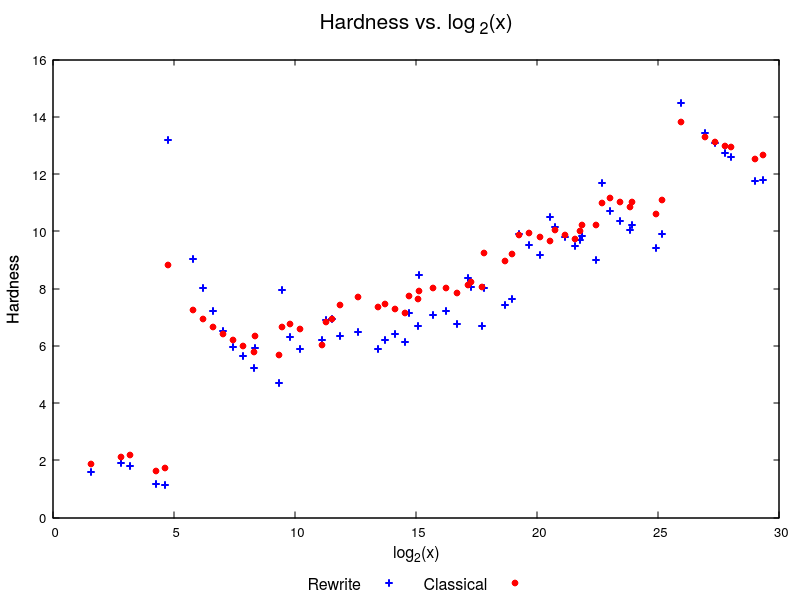
\includegraphics[scale=0.75]{ModAvoidanceAnalysisPics/RvC_vs_log.png}
    \caption{This graph compares, on the same set of input numbers, classical hardness as defined in Chapter~\ref{sec:subhrdnspred}, and rewrite hardness, which is the number of steps divided by the number of input bits squared. The number of bits for the records ($\log_2{r}$) is the x-axis, and the hardness is the y-axis.}
    \label{fig:rvc_log}
\end{figure}


\section{Collatz SRS Subproblem Analysis} \label{subsec:collatzsubproblemananalysis}
Now we know that the Collatz SRS adds a factor of $m$ more steps compared to the steps in Collatz Sequences, we look back at the Collatz Variants. In this section, we modify the Collatz SRS to create various ``Collatz Subproblems''. These subproblems are modifications of the SRRs for the Collatz SRS with the goal of having Collatz Subproblems that align with our previously defined Collatz Variants. We show how to create Collatz Subproblems, then run computation using our Collatz SRS simulation.
\subsection{Modified Base 8 Rewrite System} \label{subsec:base8rewrite}
We modified the Collatz SRS to make it tie into Collatz Variants. Recall the $D$ rules of the Collatz SRS:
\begin{align*}
    D_1: ad &\rightarrow d &\text{$0\Mod{2}$}\\
    D_2: bd &\rightarrow gd &\text{$1\Mod{2}$}\\
\end{align*}
$D_1$ handles numbers congruent modulo to $0 \Mod{2}$ by dividing the number by 2, while $D_2$ handles numbers congruent modulo to $1 \Mod{2}$  by computing $(3N+1)/2$. Also note that all input strings for these rules are just one bit, since the placeholder $d$ is not a bit.\par
We can expand the input from 1 bit to 3 bits and come up with 8 $D$ rules to create an equivalent system:
\begin{align*}
    aaad &\rightarrow aad &\text{$0\Mod{8}$}\\
    aabd &\rightarrow ebad &\text{$1\Mod{8}$}\\
    abad &\rightarrow abd &\text{$2\Mod{8}$}\\
    abbd &\rightarrow fabd &\text{$3\Mod{8}$}\\
    baad &\rightarrow bad &\text{$4\Mod{8}$}\\
    babd &\rightarrow gaad &\text{$5\Mod{8}$}\\
    bbad &\rightarrow bbd &\text{$6\Mod{8}$}\\
    bbbd &\rightarrow gbbd &\text{$7\Mod{8}$}
\end{align*}
\hl{Observe that the input substrings for these rules all correspond to a node in graph $G_8$. The rules take in substrings that represent numbers congruent modulo to 0-7$\Mod{8}$, meaning the numbers represented by the whole input strings would be visiting nodes 0-7, respectively. The outputs are the result of dividing by 2 or multiplying by 3 and adding 1, in context of the SRS.} All of the odd node rule outputs, like rule $D_2$ in the original system, are just a combination of several rules, which ensure that the output string is not longer, and it reduces a couple of steps by moving the ternary term toward the front. All of the even node rules are just the same exact rule $D_1$ in the original system, so we can remove any even rules and replace them with the original $D_1$. We can also eliminate any extra $a$ terms in the output of odd rules that we know would be eliminated by rule $D_1$. We ended up using the following SRRs in the Base 8 Collatz SRS:
\begin{align*}
    D_{8_1}: ad &\rightarrow d &\text{$0\Mod{2}$}\\
    D_{8_2}: aabd &\rightarrow ebd &\text{$1\Mod{8}$}\\
    D_{8_3}: abbd &\rightarrow fabd &\text{$3\Mod{8}$}\\
    D_{8_4}: babd &\rightarrow gd &\text{$5\Mod{8}$}\\
    D_{8_5}: bbbd &\rightarrow gbbd &\text{$7\Mod{8}$}
\end{align*}
Because these rules were constructed using only SRRs in the Collatz SRS that we know to be correct, we know these new $D$ rules, plus the $A$, $B$, and $C$ rules, are equivalent to the original Collatz SRS. However, removing one of these rules could make the system easier to prove, which in turn constructs something much like a Collatz Variant. We present such an SRS with rule $D_{8_2}$ removed:
\begin{align*}
    D_{8_1}: ad &\rightarrow d &\text{$0\Mod{2}$}\\
    D_{8_3}: abbd &\rightarrow fbbd &\text{$3\Mod{8}$}\\
    D_{8_4}: babd &\rightarrow gd &\text{$5\Mod{8}$}\\
    D_{8_5}: bbbd &\rightarrow gbbd &\text{$7\Mod{8}$}
\end{align*}
Since we removed the SRR that corresponds to input $1 \Mod{8}$, termination of this SRS \hl{should imply} termination of Collatz Variant 1, as removing a rule causes any string with this input to terminate the system. This modified Collatz SRS is called Collatz Subproblem 1 in this paper. Note how removing an SRR is equivalent to adding the corresponding termination condition in Algorithm~\ref{alg:ColSP}.  We analyzed this and other Collatz Subproblems that \hl{should imply} termination of unproven Collatz Variants.\par
\subsection{Defining Measures for Subproblem Analysis} \label{subsec:rewritemeasuredefs}
For the Collatz Subproblem computations, instead of defining hardness by number of odd numbers, we define hardness based off of the total steps applied, because of the fact that odd numbers add significantly more steps than even numbers. Define the following numbers, given some input number $N$:
\begin{itemize}
    \item $f_r(N)$: The total number of Collatz SRS rewrite steps for $N$ before it converges to 1.
    \item $A$: The base avoidance set, same as used in Algorithm~\ref{alg:ColSP} and Chapter~\ref{sec:subhrdnspred}. In this chapter, $A \subseteq \{1, 5, 7\}$ and $A \ne \varnothing$. 
    \item \hl{Collatz Subproblem $A$: Defined much in the same way as Collatz Variant $A$, but with modified Collatz SRSes instead. Let $A$ be the base avoidance set.  Collatz Subproblem $A$ is a modified Base 8 Collatz SRS that, for all $a \in A$, the SRR corresponding to $a \Mod{8}$ is removed. Therefore, any string that has the input to a dropped rule will caused the modified Collatz SRS to terminate in the same manner as Collatz Variants. Listing several Collatz Subproblems is done in the same way as Collatz Variants, so we can write Collatz Subproblems 1 and $\{5,7\}$ to mean these two modifications of the Base 8 Collatz SRS.}
    \item \hl{Record Sequence for Collatz Subproblem $A$: This is the same record sequence as for Collatz Variant $A$, which was defined in Chapter}~\ref{sec:subhrdnspred}, \hl{but we start with an input string representing the first number in the Record Collatz Variant Sequence, and run rewrite rules until we reach the number whose input string causes Collatz Subproblem $A$ to terminate (same number that causes Collatz Variant $A$ to terminate).} We only run SRSes for the record numbers we determined with the algebraic Collatz Program defined in subsection~\ref{subsec:algcomp}, as running computation for only the Collatz SRS on all odd numbers up to 1 billion would take an extremely long time.
    \item \hl{$R(N, A, 8):$ The number of rewrite steps that the record sequence for Collatz Variant $A$ for base 8 and number $N$ takes when run as Collatz Subproblem $A$ instead.}
\end{itemize}
We define a hardness measure: $H_{SRS}$, where $H_{SRS} = \frac{R(N, A, 8)}{\log_2^2{N}}$. This effectively computes the hardness of the SRRs that corresponds to determining termination of Collatz Variant $A$, but $H_{SRS}$ also takes into account the extra factor of $m$ steps that the Collatz SRS adds. The number of bits we divide by is determined by our starting number, not the first number in the record length sequence. This is the same as for our Collatz Variant computation in Chapter~\ref{sec:subhrdnspred}.

\subsection{Subproblem Hardness Analysis} \label{subsec:rewritehardness}
Figure~\ref{fig:rvslog} shows the analysis of hardness for the modified SRS with four different Collatz Subproblems: 1, 5, 7, and $\{5,7\}$. 
\begin{figure}
    \centering
    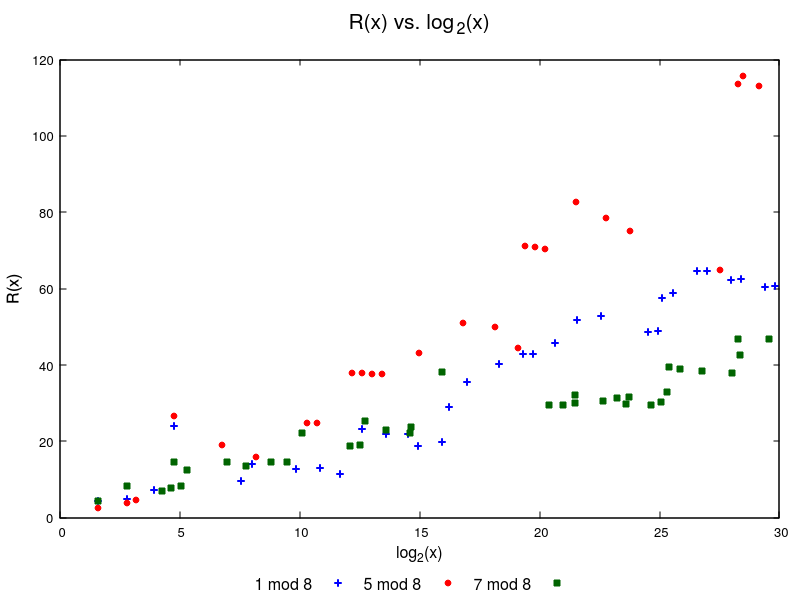
\includegraphics[scale=0.75]{ModAvoidanceAnalysisPics/R_vs_log.png}
    \caption{This graph visualizes how, for records $r$, the $R$ values for subproblems 1, 5, and 7 compare to each other. The number of bits for the records ($\log_2{N}$) is the x-axis, and the hardness measure $R$ as defined in section~\ref{subsec:rewritemeasuredefs} is the y-axis.}
    \label{fig:rvslog}
\end{figure}
Unlike the analysis for the Collatz Variants, we have clearer separation. Subproblem 5 has the highest $H_{SRS}$ on almost all of its records. Since Collatz Variant 5 record sequences tend to grow to very large numbers, these extra bits that the large numbers generate add even more steps needed by the rewrite system. Further, subproblem 5 appears to get harder as the number of bits increases, a trend not apparent in the Collatz Variant 5 $H$ measure. Subproblem 1 exhibits the growth as numbers get bigger, but tapers off once again for numbers more than 20 bits, much like Collatz Variant 1. Subproblem 7 shows no increase in $H_{SRS}$ as numbers get larger. This suggests subproblem 7 might be easier to solve than subproblems 1 or 5. Subproblem $\{5,7\}$ has the lowest hardness, which makes sense given that it has one less rule than any of the other three subproblems.
\section{Further SRS Rule Modifications}\label{subsec:srsrulemod}
It is possible that the set of SRRs in the Collatz SRS can be optimized to reduce number of rewrite steps. These optimizations may possibly lead to solutions for the subproblems listed in this chapter. We present one modification of the Collatz SRS by replacing the base $D$ rules with rules that have both input and output correspond to odd numbers. We then look at the results of doing so.
\subsection{Odd Collatz SRS}\label{subsubsec:evenruleremove}
It is possible to replace both $D_1$ and $D_2$ in the Collatz SRS with the following set of rules that calculates with strictly odd numbers:
\begin{align*}
    D_{o1}: bbd &\rightarrow gbd &\text{$3\Mod{4}$}\\
    D_{o2}: aabd &\rightarrow ebd &\text{$1\Mod{8}$}\\
    D_{o3}: babd &\rightarrow bd &\text{$5\Mod{8}$}
\end{align*}
Notice that rule $D_{o1}$ and $D_{o2}$ are borrowed from the base 8 modification of the Collatz SRS. $D_{o1}$ combines both rule $D_{8_3}$ and $D_{8_5}$, removing the leading $a$ or $b$, respectively. $D_{o1}$ has the $A$, $B$, and $C$ rules determine the next symbol(s). Rule $D_{o2}$ is the same as rule $D_{8_2}$.\par
Rule $D_{o3}$ is not as intuitive at first glance, but we can look at rule $D_{8_4}$, which has the same input as $D_{o3}$, and see that the output for $D_{8_4}$ is the same as the normal $D_2$ rule, $gd$, so we can ``step backwards'' using rule $D_2$ to allow for us to get $bd$ as our output, and hence, have a full set of correct $D$ rules that go from odd number to odd number.\par
Observe that all of the $D_o$ rules have a left handed side and a right handed side ending with $bd$. As a consequence, we can remove the $b$ symbol in the second to last symbol for both the input string and the rules, resulting in the following SRRs:
\begin{align*}
    D_{o1^*}: bd &\rightarrow gd &\text{$3\Mod{4}$}\\
    D_{o2^*}: aad &\rightarrow ed &\text{$1\Mod{8}$}\\
    D_{o3^*}: bad &\rightarrow d &\text{$5\Mod{8}$}
\end{align*}
\subsection{Change in Rewrite Steps}
\begin{figure}
    \centering
    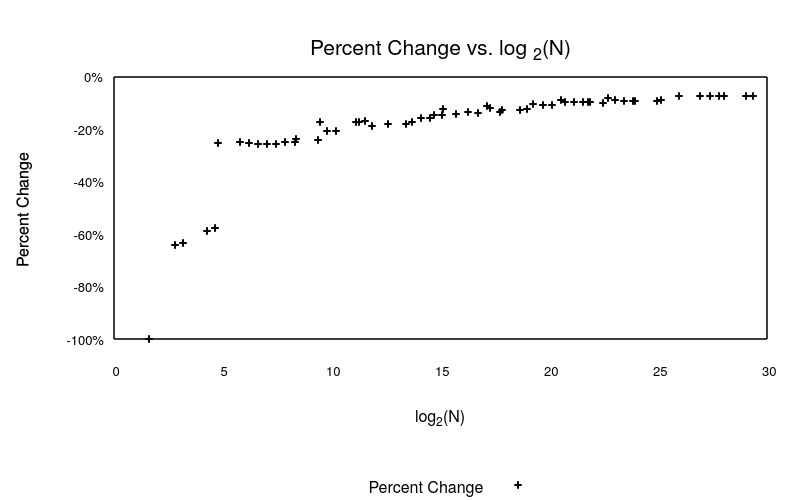
\includegraphics[scale=0.75]{ModAvoidanceAnalysisPics/Percent_Change.png}
    \caption{This graph shows what percentage the odd rules change the rewrite steps, as opposed to the original Collatz SRS. The number of bits for the records ($\log_2{N}$) is the x-axis, and the percent decrease is the y-axis.}
    \label{fig:percent_decrease}
\end{figure}
Figure~\ref{fig:percent_decrease} \hl{shows the percentage of rewrite steps the Odd Collatz SRS changes, compared to the original Collatz SRS, when run on classical hardness records. The Odd Collatz SRS reduces the number of steps greatly for smaller numbers. However, as the numbers get larger, the percentage reduction of steps lowers significantly. This is probably because records for larger numbers have $3N+1$ sequences that tend to have more odd numbers, which add in more rewrite steps.} That said, this modification to the rewrite system does overall reduce the number of rewrite steps. Other SRR modifications for the Collatz SRS should be considered, as the right set of clever rules may prove termination of Collatz Subproblems, and perhaps, even prove that the Collatz Conjecture holds.


%  shows the percentage change for classical hardness records when the $D_o$ rules are used compared to the normal $D$ rules. Lower numbers tend to have a larger percentage of decrease, but as the numbers get larger, the decrease percentage reduces by quite a bit. This is probably because records for larger numbers tend to have more odd numbers, meaning many more rewrite steps than lower numbers. 

%%  LocalWords:  SRS Heule's SRSes SRR SRRs GitHub readme Subproblem
%%  LocalWords:  Subproblems subproblems bd gd aaad aad aabd ebad abd
%%  LocalWords:  abad abbd fabd baad babd gaad bbad bbd bbbd gbbd ebd
%%  LocalWords:  substrings fbbd subproblem optimizations gbd
